\documentclass{article}
\usepackage[utf8]{inputenc}
\usepackage{subfig}

%References
\usepackage{natbib}
%IMPORTANT use https://www.citationmachine.net/ if you need to generate references!
% \citep{reference} creates Harvard Style references throughout

%Colors
\usepackage{xcolor}

\usepackage[protrusion=true,expansion]{microtype}

%Code Markup
\usepackage[outputdir=cache]{minted}
%Syntax Highlighting Style
\definecolor{bggray}{RGB}{40,40,40}
\newmintedfile[javacode]{java}{
	style=fruity,
	bgcolor=bggray,
	linenos,
	breaklines,
	tabsize=2,
	obeytabs
}

\newmintedfile[bashoutput]{text} {
	style=fruity,
	bgcolor=bggray,
	breaklines,
	tabsize =2,
	obeytabs
}

\newmintedfile[armfile]{ARM} {
	style=fruity,
	bgcolor=bggray,
	breaklines,
	tabsize =2,
	obeytabs
}

%Page Margins and stuff
\usepackage{geometry}
 \geometry{
 a4paper,
 total={170mm,257mm},
 left=20mm,
 }

%Pictures
\usepackage{graphicx}
\graphicspath{ {./images/} }

%Move the title position
\usepackage{titling}

\setlength{\droptitle}{-8.5em} %Up, near the top but not too high

\title{Lab Exercise 5 - CT213 Computer Systems \& Organizaton}
\author{Daniel Hannon (19484286)}
\date{December 2020}

\begin{document}
	\maketitle
	\section{Part 2}
	\armfile{addfloat.s}
	\begin{figure}[h!]
		\centering
		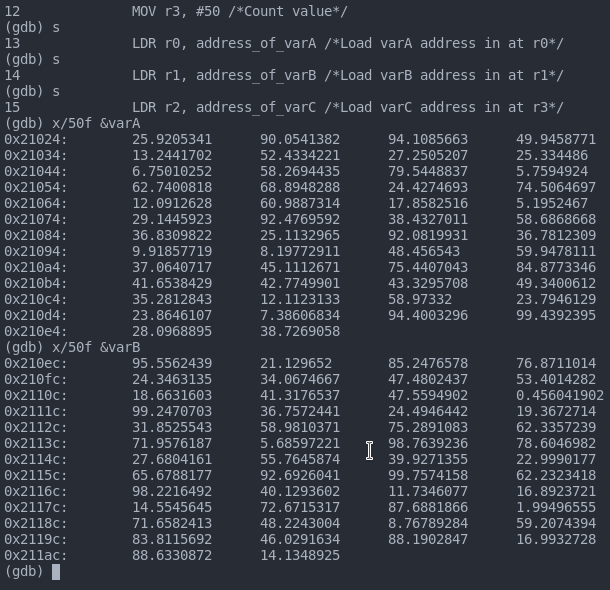
\includegraphics[width=0.8\textwidth]{varA_varB.png}
		\caption{VarA/B contents}
	\end{figure}
	\begin{figure}[h!]
		\centering
		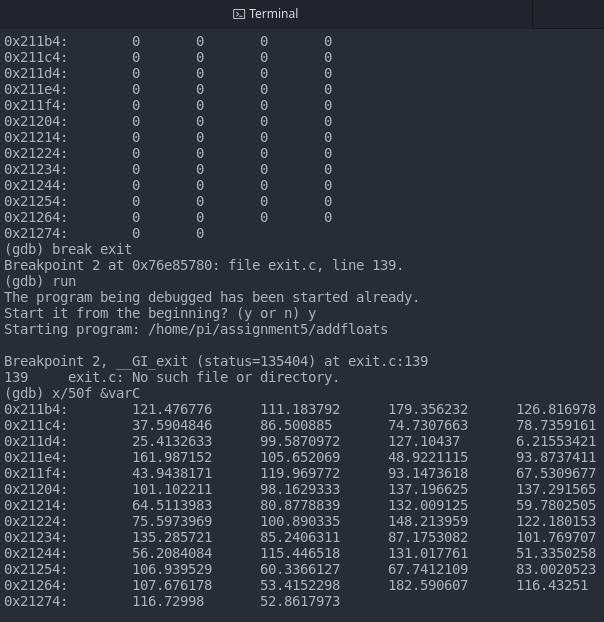
\includegraphics[width=0.8\textwidth]{VarC_before_after.png}
		\caption{VarC before/after running}
	\end{figure}
	%Sets to Harvard Style and links the references file
	\bibliographystyle{agsm}
	\bibliography{references}
\end{document}
